\documentclass{article}

%other packages
\usepackage[a4paper]{geometry}
\usepackage{longtable}
\usepackage{wrapfig}
\setlength\parindent{0pt}
\usepackage{enumitem}
\usepackage[table,dvipsnames]{xcolor}
\usepackage{polynom}
\def\scaleint#1{\vcenter{\hbox{\scaleto[3ex]{\displaystyle\int}{#1}}}}
\usepackage{array}
\newcolumntype{C}{>{{}}c<{{}}} % for '+' and '-' symbols
\newcolumntype{R}{>{\displaystyle}r} % automatic display-style math mode 
\usepackage{tabularray}
\usepackage{dcolumn,tabularx,booktabs}
\usepackage[most]{tcolorbox}

%maths
\usepackage{mathtools}
\usepackage{amsmath}
\usepackage{amssymb}
\usepackage{amsfonts}
\usepackage{autobreak}

%tikzpicture
\usepackage{tikz}
\usepackage{scalerel}
\usepackage{pict2e}
\usepackage{tkz-euclide}
\usepackage{tikz-3dplot}
\usetikzlibrary{calc}
\usetikzlibrary{patterns,arrows.meta}
\usetikzlibrary{shadows}
\usetikzlibrary{external}
\usetikzlibrary{decorations.pathreplacing,angles,quotes}

%pgfplots
\usepackage{pgfplots}
\pgfplotsset{compat=1.18}
\usepgfplotslibrary{statistics}
\usepgfplotslibrary{fillbetween}

\pgfplotsset{
    standard/.style={
    axis line style = thick,
    trig format=deg,
    enlargelimits,
    axis x line=middle,
    axis y line=middle,
    enlarge x limits=0.15,
    enlarge y limits=0.15,
    every axis x label/.style={at={(current axis.right of origin)},anchor=north west},
    every axis y label/.style={at={(current axis.above origin)},anchor=south east}
    }
}

\begin{document}

Math 115 - Week 4, Class 10 - 24 Jan 2024
\hrule

\vspace{10pt}

There was a question about the example from last class when we were asked to evaluate $\sin(2\arctan3)$, and Dr. Solomonovich went over a particular point on the board - since we already went over this, we will omit it.

\vspace{10pt}

The trigonometry formulae are important. Some are easy to derive, some are not. Even if we can't derive them, we still need to know them.

\begin{align*}
\sin(x+y)&=\sin x\cos y+\sin y\cos x\\
\cos(x+y)&=\cos x\cos y-\sin x\sin y\\
\tan(x+y)&=\frac{\sin x\cos y+\sin y\cos x}{\cos x\cos y-\sin x\sin y}\\
&=\frac{\frac{\sin x\cos y}{\cos x\cos y}+\frac{\sin y\cos x}{\cos x\cos y}}{1-\frac{\sin x\sin y}{\cos x\cos y}}\\
&=\frac{\tan x\tan y}{1-\tan x\tan  y}
\end{align*}

\vspace{10pt}

To differentiate the arctangent function, we do the following;

\begin{align*}
y&=\arctan x\\
&=\left\{\begin{array}{c}x=\tan y\\|y|<\pi/2\end{array}\right.\\
y^\prime&=\frac{dy}{dx}=\frac{1}{\left(\frac{dx}{dy}\right)}\\
&=\frac{1}{\left(\frac{1}{\cos^2y}\right)}\\
&=1\div\frac{1}{\cos^2y}=\cos^2y\\
\mbox{And we know }\sin^y+\cos^2y&=1\\
\mbox{So, }\tan^2y+1&=\frac{1}{\cos^2y}\\
\mbox{And }\cos^2y&=\frac{1}{1+\tan^2y}\\
\mbox{Therefore, }(\arctan x)^\prime&=\frac{1}{1+x^2}
\end{align*}

\vspace{10pt}

Dr. Solomonovich also wants us to solve for $(\mbox{arccot }x)^\prime$ on our own time using similar methods. He says that even though we will never use it that we should still be able to derive it. He also mentioned that it is important to know the derivatives of inverse sine and cosine, as well as the following few formulas;

\begin{align}
\arcsin x+\arccos x&=\frac{\pi}{2}\\
\int\frac{1}{\sqrt{a^2-x^2}}\ dx&=\arcsin\frac{x}{a}+C\\
\int\frac{1}{a^2+x^2}\ dx&=\frac{1}{a}\arctan\frac{x}{a}+C
\end{align}

\vspace{10pt}

We then solved a problem where we used a substitution to manipulate the integrand into a form which could be solved using the technique we just learned.

\begin{align*}
\int\frac{e^{2x}}{1-e^{4x}}\ dx&=\left|\begin{array}{c}e^{4x}=(e^{2x})^2\\de^{2x}=2e^{2x}\ dx\end{array}\right.\\
&=\left(\begin{array}{cl}e^{2x}=t &e^{4x}=t^2\\2e^{2x}\ dx=dt&\\
e^{2x}\ dx=\frac{1}{2}\ dt&\end{array}\right)\\
&=\frac{1}{2}\int\frac{dt}{\sqrt{1-t^2}}\\
&=\frac{1}{2}\arcsin t+C\\
&=\frac{1}{2}\arcsin e^{2x}+C
\end{align*}

\vspace{10pt}

Then we did a similar exercise where we looked for $\displaystyle\int_0^{\pi/2}\frac{\sin x}{1+\cos^2x}\ dx$

\vspace{10pt}

So we recognize that there is a derivative-antiderivative pair of terms present in a way where if we perform the corresponding substitution, then we would be left with an integrand of an integrable form. More cool however is the use of differential notation; this will be useful in trigonometric inverse-substitution integrals later on in the course, where you will need to substitute entire expressions for the differential.

\[\sin x\ dx=-d\ \cos x\]

\[\begin{array}{cc}(x^2)^\prime=2x&d\ x^2=2\ dx\\
(\sqrt{x})^\prime=\frac{1}{2\sqrt{x}}&d\ \sqrt{x}=\frac{1}{2\sqrt{x}}\ dx\end{array}\]

\vspace{10pt}

Anyway, back to the question;

\begin{align*}
\int_0^{\pi/2}\frac{\sin x}{1+\cos^2x}\ dx&=\left(\begin{array}{c}\cos x=t\\d\ \cos x=\sin x\ dx\\\sin x\ dx=-\ dt\end{array}\right.\\
&=\int_1^0\frac{-\ dt}{1+t^2}\quad\mbox{ s.t. }\quad-\int_a^b=\int_b^a\\
&=\int_0^1\frac{dt}{1+t^2}=\arctan t\Big|_0^1\\
&=\arctan1-\arctan0\\
&=\frac{\pi}{4}-0=\frac{\pi}{4}
\end{align*}

\vspace{10pt}

We moved onto some hyperbolic functions. Hyperbolic functions are just like trigonometric functions,  but for hyperbolas; that is, the sine hyperbolic and cosine hyperbolic functions output the vertical and horizontal projections respectively of the radial line which intersects the hyperbola - the area of the region enclosed by this line, the hyperbola, and the coordinate axis is half the paramater. Hyperbolas are defined as this: $x^2-y^2=a^2$.

\begin{center}
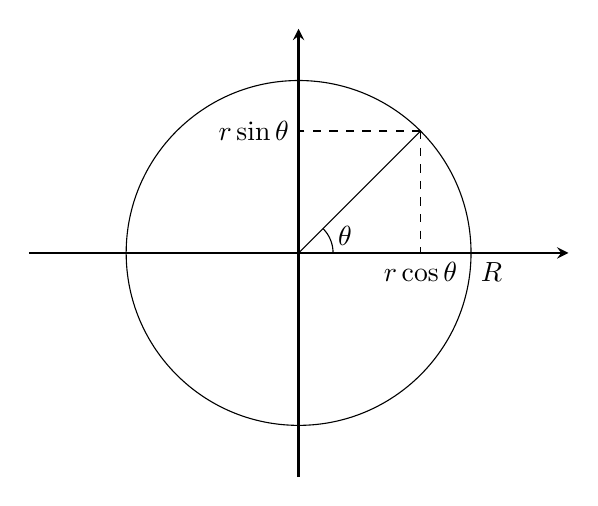
\begin{tikzpicture}
\begin{axis}[
standard,
xmin=-1, xmax=1,
ymin=-1, ymax=1,
axis equal,
xtick={\empty}, ytick={\empty}]
\draw[] (0,0) circle [radius=1];
\node[below right] at (1,0) {$R$};
\draw[] (0,0) -- (45:1);
\draw[dashed] (45:1) -- (45:1 |- 0,0) node[pos=1, below] {$r\cos\theta$};
\draw[dashed] (45:1) -- (45:1 -| 0,0) node[pos=1, left] {$r\sin\theta$};;
\draw[] (0.2,0) arc [start angle=0, end angle=45, radius=0.2];
\node[right] at (30:0.2) {$\theta$}; 
\end{axis}
\end{tikzpicture}
\hspace{20pt}
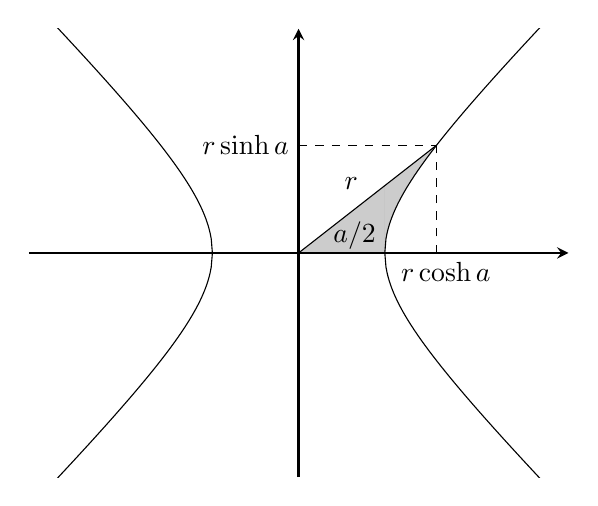
\begin{tikzpicture}
\begin{axis}[
standard,
xmin=-2, xmax=2,
ymin=-2, ymax=2,
axis equal,
xtick={\empty}, ytick={\empty}]
\addplot[samples=300,domain=1:5, name path=G] {(x^2-1)^(1/2)};
\addplot[samples=300,domain=1:5] {-(x^2-1)^(1/2)};
\addplot[samples=300,domain=-1:-5] {(x^2-1)^(1/2)};
\addplot[samples=300,domain=-1:-5] {-(x^2-1)^(1/2)};
\path[name path=H] (0,0) -- (1,0);
\draw[name path=F] (0,0) -- (1.6,1.24936) node[pos=0.5, above left] {$r$};
\addplot[fill=black, fill opacity=0.2] fill between [of=F and G, soft clip={domain=1:1.6}];
\addplot[fill=black, fill opacity=0.2] fill between [of=F and H, soft clip={domain=0:1}];
\node[] at (0.65,0.2) {$a/2$};
\draw[dashed] (0,1.24936) -- (1.6,1.24936) node[pos=0, left]{$r\sinh a$};
\draw[dashed] (1.6,0) -- (1.6,1.24936) node[pos=0, below]{$\ \ r\cosh a$};
\end{axis}
\end{tikzpicture}
\end{center}

\vspace{10pt}

And these are the relevant definitions, though they will not be on the test.

\begin{align}
\sinh x&=\frac{e^x-e^{-x}}{2}\\
\cosh x&=\frac{e^x+e^{-x}}{2}\\
\tanh x&=\frac{\sinh x}{\cosh x}\\
\coth x&=\frac{\cosh x}{\sinh x}
\end{align}

\vspace{10pt}

Then we derived a useful formula for hyperbolic tangent;

\begin{align*}
\tanh x&=\frac{e^x-e^{-x}}{e^x+e^{-x}}\\
&\overset{\div e^{-x}}{\underset{\frac{e^x}{e^{-x}}=e^{2x}}{=\joinrel=\joinrel=\joinrel=\joinrel=\joinrel=}}\frac{e^{2x}-1}{e^{2x}+1}
\end{align*}

\vspace{10pt}

And these hyperbolic functions have identities similar to the trigonometrics; for instance,

\[\cosh^2x-\sinh^2x=1\]

\vspace{10pt}

Which can be proves by arithmetically working it out from the definition.




\end{document}